\documentclass[11pt]{article} 
\usepackage[american]{babel}
\usepackage{makeidx}
\usepackage{amssymb}
\usepackage{amsmath}
\usepackage{xfrac}
\usepackage{graphicx}
\usepackage{amsthm}
\usepackage{caption}
\usepackage{subcaption}

\oddsidemargin= -12pt \evensidemargin= -12pt
\topmargin=-45pt
\binoppenalty=10000
\relpenalty=10000
\textwidth=6.5in\textheight=9in \baselineskip=18pt
\parskip=6pt plus 1pt
\numberwithin{equation}{section}

\newtheorem{proposition}{Proposition}[section]

\begin{document}

\begin{center} 
\Large {Tel-Aviv University}

\Large {The Raymond and Beverly Sackler Faculty of} \\
\Large {Exact Sciences} \\
\Large {The Department of Statistics and Operations} \\
\Large {Research}

\bigskip
\bigskip
\bigskip

\Large {\bf Draft }

\bigskip
\bigskip
\bigskip
\bigskip

\Large{Thesis Submitted Towards the Degree of Master} \\
\Large {of Science in Operations Research}

\bigskip

\Large {Ran Snitkovsky}

\bigskip
\bigskip
\bigskip

\Large {Supervisor:} \\
\Large {Prof. Refael Hassin}

\bigskip
\bigskip

\Large{2014}

\end{center}

\newpage

\begin{center} \Large {\bf Draft}
\end{center}

\begin{abstract} 

To-do...

\newpage

\end{abstract}

\section{Introduction}

To-do...

\newpage

\section{System-model}

We consider a system composed of two identical servers, $S_{1}$ and $S_{2}$, each one's service-duration is exponential with rate $\mu$, and a single FCFS unobservable queue (see Fig.\ref{CostumersFlow}). Costumers are identical, and arrive at the system following a Poisson-process with rate $\Lambda$. Upon his arrival, a costumer chooses one between two options: pay a 'sensing-price' and try to attain service in $S_{2}$ (a.k.a, 'Sense'), or, join the queue and wait until accepted to service in $S_{1}$ (a.k.a 'Not-Sense'). A costumer who chooses to sense $S_{2}$ and finds it idle, is immediately accepted to service without waiting. However, if he finds $S_{2}$ occupied, he is sent to the queue and waits his turn to service by $S_{1}$.

Denote $p$ the probability that a costumer senses $S_{2}$, and denote $(X_{1}(t), X_{2}(t))$ the state of the system at time $t$, consisting of the number of costumers in the queue (including the one in service at $S_{1}$) and the state of $S_{2}$ respectively, with $X_{1}(t) \in \lbrace0, 1, 2, \ldots\rbrace$ and $X_{2}(t) \in \lbrace0, 1\rbrace$ (0 means that $S_{2}$ is idle). Thus, the system can be described as a bi-dimensional Markov process, as shown in Fig.\ref{MarkovChain}, and the stationary probabilities are computed through the following set of equations: 

\begin{equation}
  \begin{cases}
    \Lambda P_{0,0} - \mu P_{1,0}  - \mu P_{0,1} = 0\\
    (\mu+\Lambda) P_{0,1} - p\Lambda P_{0,0}  - \mu P_{1,1} = 0
  \end{cases}
	\label{StateEq1}
\end{equation}

\begin{equation}
  \forall n \in \lbrace 1, 2, \ldots \rbrace: \ \begin{cases}
    (\mu+\Lambda) P_{n,0} - (1-p) \Lambda P_{n-1, 0} - \mu P_{n+1,0}  - \mu P_{n,1} = 0\\
    (2\mu+\Lambda) P_{n,1} - p\Lambda P_{n,0}  - \Lambda P_{n-1,1} - \mu P_{n+1,1} = 0
  \end{cases} \label{StateEq2}
\end{equation}
where $P_{i,j}$ is the stationary probability that the system is in state $(i,j)$. These equations induce the following relationship:

\begin{equation}
  \forall n \in \lbrace 0, 1, 2, \ldots \rbrace: \ 
    P_{n+1,0} + P_{n+1,1} = \dfrac{\Lambda}{\mu}((1-p) P_{n,0} +  P_{n, 0}) \label{RecurtionRule}
\end{equation}

By the assumption that each individual chooses randomly and independently whether to sense or not, we deduce that the sub-system $S_{2}$ can be considered as an M/M/1/1 queue (Erlang's Loss Model) with arrival rate $p\Lambda$ and service rate $\mu$. Therefore, the 'loss-probability' of $S_{2}$ (a.k.a the probability that a costumer sensing $S_{2}$ will find it occupied) is:
\begin{equation}
	Pr(X_2=1) = \sum\limits_{i=0}^{\infty} P_{i, 1} = \dfrac{p\Lambda}{\mu+p\Lambda} \label{LossProb}
\end{equation}
and it's complement:
\begin{equation}
	Pr(X_2=0) = 1-Pr(X_2=1) = \sum\limits_{i=0}^{\infty} P_{i, 0} = \dfrac{\mu}{\mu+p\Lambda} \label{OMLossProb}
\end{equation}
One can also derive the above formula by summing the right-hand-sides of the equations in (\ref{RecurtionRule}) for $n=0,1,2,\ldots$ and comparing the sum of this infinite series to $1-(P_{0,0}+P_{0,1})$, considering that in steady state of the system it holds: \[ p\Lambda\sum_{i=0}^{\infty}P_{i,0} - \mu \sum_{i=0}^{\infty}P_{i,1} = 0\]

Summing the equations in (\ref{RecurtionRule}) for $n=0,1,2,\ldots$ and substituting (\ref{LossProb}) and (\ref{OMLossProb}) we get:

\begin{equation}
	P_{0,0} + P_{1,0} = 1- \frac{ \Lambda}{ \mu}\left(1- \frac{p}{1+p \frac{\Lambda}{\mu}} \right) \label{P00PlusP01}
\end{equation}
which induces a linear relationship between $P_{0,0}$ and $P_{0,1}$.

Subtracting the second equation from the first one in (\ref{StateEq2}) and combining (\ref{RecurtionRule}) we deduce the following formulae:
\begin{equation}
	\forall n \in \lbrace 0, 1, \ldots \rbrace: \
  	\begin{cases}
    	P_{n+1,0} = (1-p) \frac{\Lambda}{\mu} P_{n, 0} + p \frac{\Lambda}{\mu} \sum\limits_{i=0}^{n}P_{i,0} - \sum\limits_{i=0}^{n}P_{i,1}\\
   	 	P_{n+1,1} = \frac{\Lambda}{\mu} P_{n, 1} + \sum\limits_{i=0}^{n}P_{i,1} - p \frac{\Lambda}{\mu} \sum\limits_{i=0}^{n}P_{i,0}
  	\end{cases} \label{Forms}
\end{equation}
It can be seen from (\ref{Forms}) that, for given constants $p$ and $\sfrac{\Lambda}{\mu}$, every value $P_{n+1,k}$ ($k\in\lbrace0,1\rbrace$) is expressed as a linear combination of $\lbrace P_{n,0}, P_{n-1,0}, \ldots, P_{0,0}, P_{n,1}, P_{n-1,1}, \ldots, P_{0,1},  \rbrace$, hence, with (\ref{P00PlusP01}), it follows by induction that for each $n \in \lbrace 0, 1, \ldots \rbrace$ and for each $k \in \lbrace 0, 1 \rbrace$, $P_{n,k}$ is, as a composition of linear functions, a linear function of $P_{0,0}$ . Thus, for $N$ sufficiently large, one can bound the queue length by $N$, express the finite series $\sum_{i=0}^{N} P_{i,0}+P_{i,1}$ as a linear function of $P_{0,0}$, equate to 1 and find a fixed value of $P_{0,0}$ (and all other $P_{n,k}$) in $O(N)$ time complexity.
\newpage

\section{System-throughput}
We now intend to find the maximum throughput of the system. For convenience we use the notation $\rho:=\sfrac{\Lambda}{\mu}$. The 'effective-throughput' of the queue $\tilde{\rho}(p,\rho)$, meaning the effective arrival rate divided by the service rate, consists of two groups of arrivals: costumers who join the queue without sensing at all (whose proportion is $1-p$) and costumers who sense $S_{2}$ and find it busy (whose proportion is $p \cdot Pr(X_2=1)$). Therefore,
\begin{equation}
	\tilde{\rho}(p,\rho) = (1-p)\rho + \frac{p\rho}{1+p\rho}\cdot p\rho = \rho - \frac{1}{1+p\rho}p\rho \label{EffectiveRate}
\end{equation}
which is a monotone decreasing function in $p$ for every $\rho\in(0,\infty)$. 

The stochastic process representing the sequence of arrivals over time to the queue served by $S_{1}$ is not poissonian. This is because the inter-arrival times in the queue depend on the decision of each costumer whether he senses or not, and, if does so, whether he's accepted to immediate service. Thus, we model this sub-system as a G/M/1 with unnecessarily independent inter-arrival times, and for the system to remain stable we demand $\tilde{\rho}(p,\rho) < 1$, or equivalently:
\[ p>\frac{\rho - 1}{\rho(\rho-2)} \]

\begin{proposition}
For each $\rho\in(0,\varphi)$, there exists a value of $p$ for which the system is stable, where
$\varphi \approx 1.618$ is the golden ratio.
\end{proposition}

\begin{proof}
Finding the maximum throughput we assume that $p=1$, which means everyone try to attain service in $S_{2}$ before they join the queue. This is followed by the monotonicity of $\tilde{\rho}(p,\rho)$. Then, from (\ref{EffectiveRate}), the stability criterion is:
\[ \tilde{\rho}(1,\rho)=\frac{\rho^2}{1+\rho}<1 \quad\Leftrightarrow\quad \rho^2-\rho-1<0 \quad\Leftrightarrow\quad \rho < \frac{1+\sqrt{5}}{2}=\varphi \]
where $\varphi$ is the well-studied golden ratio, concluding that for every $\rho\in(0,\varphi)$ and $p=1$, the system is stable.
\end{proof}

\newpage
\section{Equilibrium Strategy}
In this section we discuss the states and strategies of (Nash) equilibrium in the system. Let $c_{w}>0$ be the time-expense for a single time unit of an individual costumer waiting in line, and $c_{s}>0$ be the price of sensing (paid by each costumer who chooses to sense, regardless of the consequences of his action). Since all costumers are identical, so are their equilibrium strategies. In addition, each one arriving at the system is eventually attained to service, and therefore, neither the reward from service nor the time spent in service is relevant. Of course, the state of the system, including the length of the queue and the status of the servers, is unobservable as mentioned, and unknown to the costumer at the time he makes his decision. We assume the system is not over-loaded (i.e: $\rho<\varphi$) and that all costumers act to reduce their expected cost to minimum. Denote $C_{S}(p)$ and $C_{N}(p)$ the expected cost of an individual who chooses to sense and an individual who chooses not to sense, respectively, as the others' probability of sensing is $p$.
\begin{equation}\begin{cases}
 	C_{N}(p) = \frac{c_{w}}{\mu}E(L(p)) \\
	C_{S}(p) = c_{s} + Pr(X_2=1) \cdot C_{N}(p) = c_{s} + \frac{p\Lambda}{\mu+p\Lambda}\frac{c_{w}}{\mu}L(p) 
\end{cases}
\label{LossFunc}
\end{equation}
where $L(p)$ is the expected queue length with $p$ the proportion of the population that sense. Denote $\gamma :=\sfrac{c_{w}}{\mu c_{s}}$. The value of $\sfrac{1}{\gamma}$ can be interpreted as the normalized cost of sensing in terms of the cost of waiting a single service period, that is to say, for how many service completions one has to wait, on average, in order to pay a total time expense of $c_{s}$. Then:

\begin{proposition} For every $\rho\in(0,\varphi)$, and for every value  $\gamma>0$, a unique equilibrium strategy $p_{e}\in[0,1]$ exists.
\end{proposition}

\begin{proof}

$p$ is an equilibrium strategy if no individual can benefit from choosing any alternative strategy. Thus, for $p$ to be an equilibrium, it must hold that $C_{N}(p)=C_{S}(p)$. Divide both sides of the latter equation by $c_{s}$ and substitute the values in (\ref{LossFunc}) to get:

\[ C_{N}(p) = C_{S}(p) \quad\Leftrightarrow\quad \gamma L(p) = 1 + \frac{p \rho}{1 + p\rho} \gamma L(p) \quad\Leftrightarrow\quad \gamma L(p)=1+p\rho \]

Note that the function $L(p)$ is continuous and strictly monotone decreasing in $p$, and therefore if there exists a solution to the equation then it is unique. Suppose that \[\forall p \in [0,1]: C_{N}(p) > C_{S}(p)\] then sensing is a dominant strategy for each individual and $p_{e}=1$. Similarly, if \[\forall p \in [0,1]: C_{N}(p) < C_{S}(p)\] then $p_{e}=0$.

\end{proof}

This result is not as intuitive as it seems, since the function $L_{S}(p)$ is not necessarily monotonic (as shown in Fig. \ref{cost_vs_p_2_05} and \ref{cost_vs_p_05_085}). This fact can be explained as follows: an increase in the proportion of costumers that sense, results in a decrease of the probability to attain service in $S_{2}$ on the first hand. It also decreases the expected queue length, and shortens the waiting time of the costumers who failed to attain $S_{2}$ on the other hand. Nevertheless, the equilibrium probability $p_{e}$ is always unique.

Suppose now that $p=0$, and $\tilde{\rho}(0,\rho) = \rho < 1$. This is an equilibrium strategy if and only if:
\[ \gamma X(0)-1 \leq 0 \]

Note that in this case the queue is a regular M/M/1 queue, and $L(p)|_{p=0} = \sfrac{\rho}{1-\rho}$. Thus, a necessary and sufficient condition for $p_{e}=0$ is:

\[ \gamma \frac{\rho}{1-\rho}-1 \leq 0 \quad\Leftrightarrow\quad \rho \leq \frac{1}{1+\gamma} \]

\newpage
\begin{figure}[h!]
    \centering
    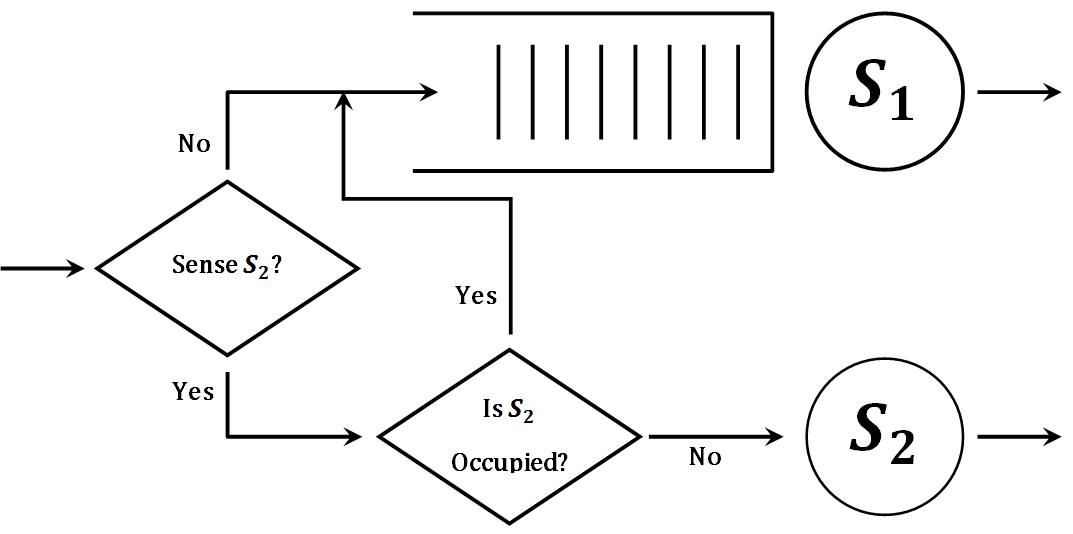
\includegraphics[width=1\textwidth]{Fig_1.png}
    \caption{Costumers' flow chart of the system with an opportunistic sensing}
    \label{CostumersFlow}
\end{figure}

\begin{figure}[h!]
  \centering
    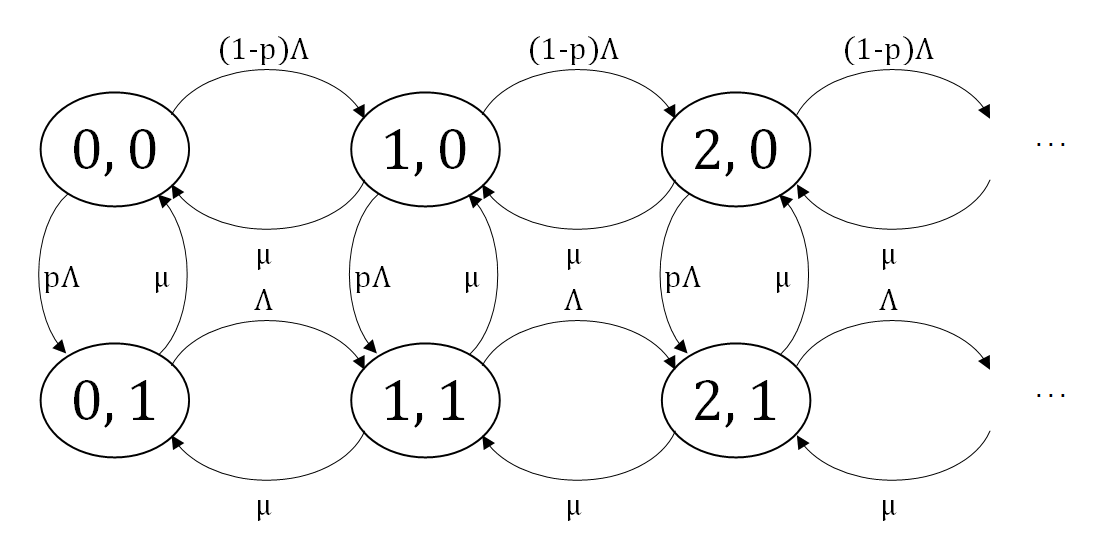
\includegraphics[width=1\textwidth]{Fig_2.png}
    \caption{The Markov chain describing the transitions between states in the system}
    \label{MarkovChain}
\end{figure}

\begin{figure}[h!]
  \centering
    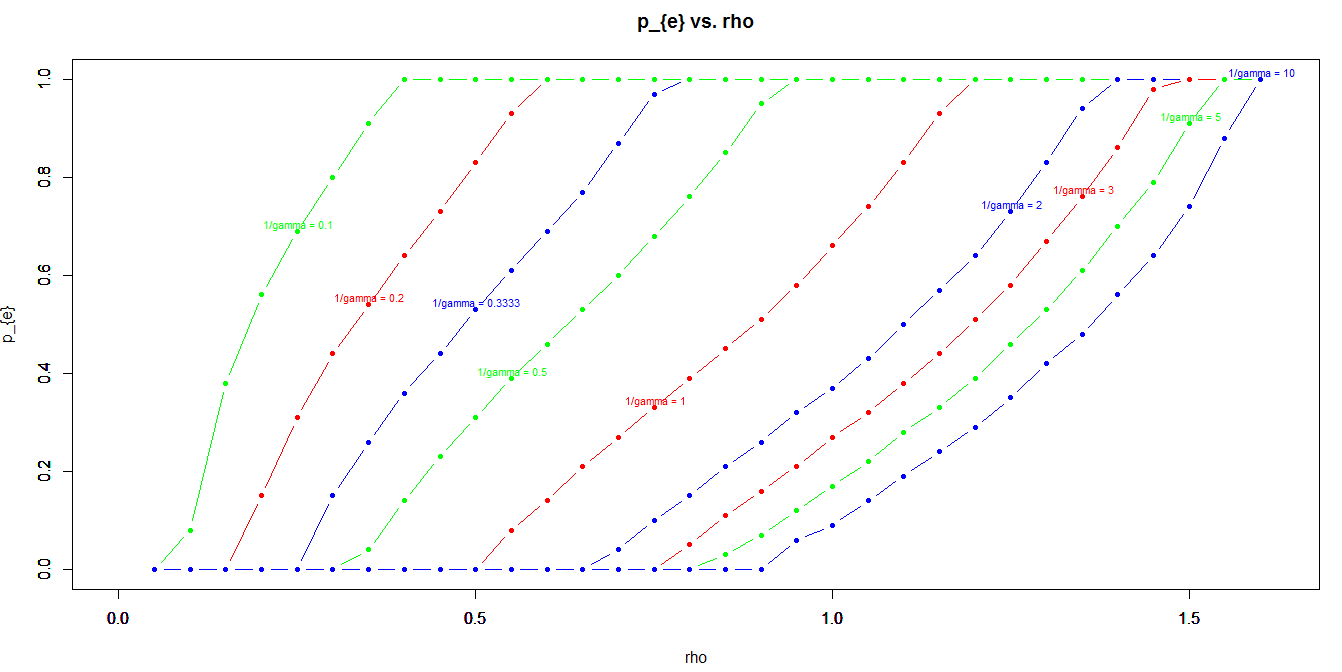
\includegraphics[width=1\textwidth]{peq_vs_rho.png}
    \caption{The equilibrium strategy $p_{e}$ as a function of $\rho$ for a various values of $\gamma$}
    \label{PeqVsRho}
\end{figure}

\begin{figure}[h!]
	\centering
	\begin{subfigure}[b]{0.49\textwidth}
		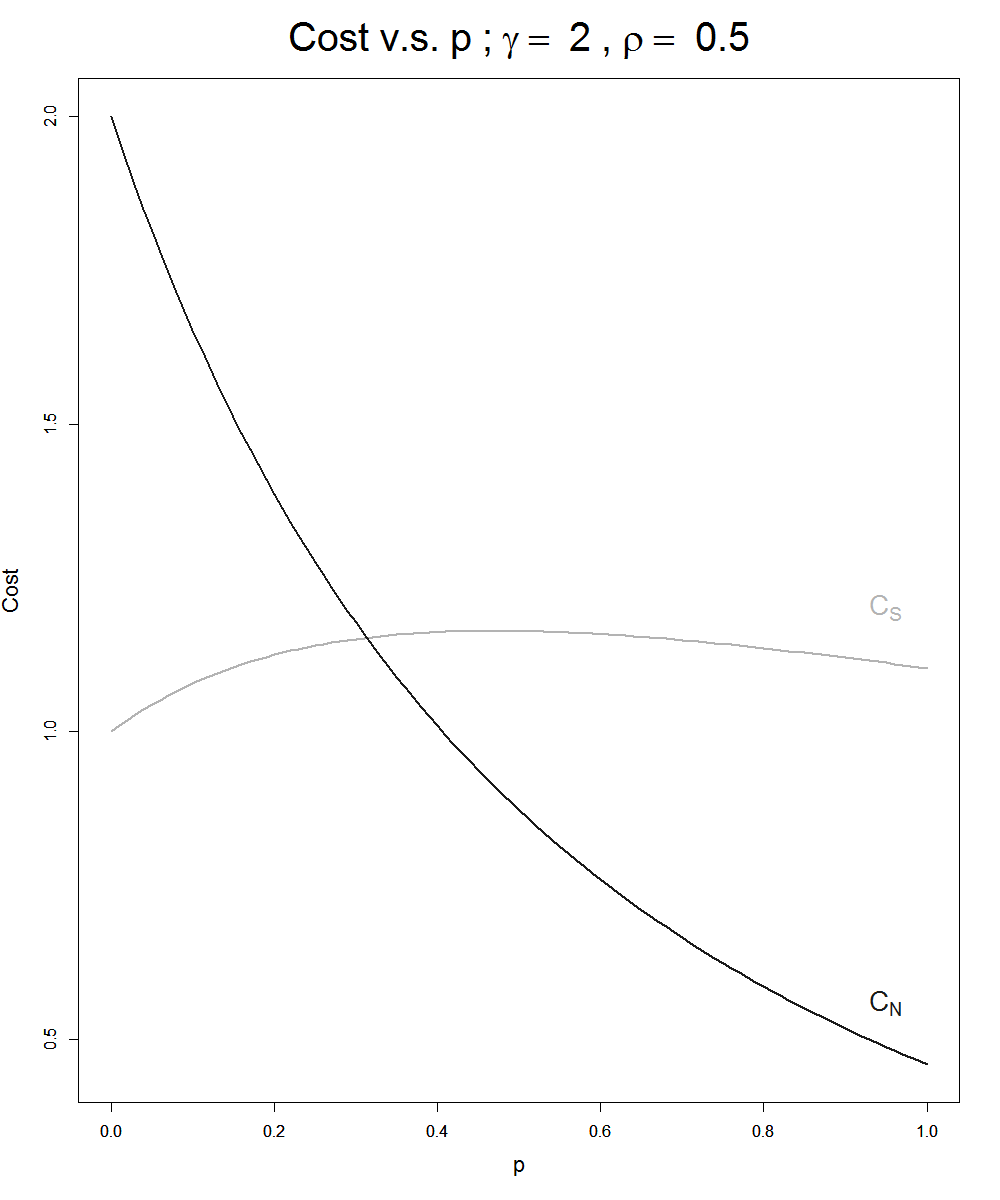
\includegraphics[width=\textwidth]{cost_vs_p_2_05}
		\caption{$\gamma=2;\quad\rho=0.5$}
	\label{cost_vs_p_2_05}
	\end{subfigure}
	\begin{subfigure}[b]{0.49\textwidth}
	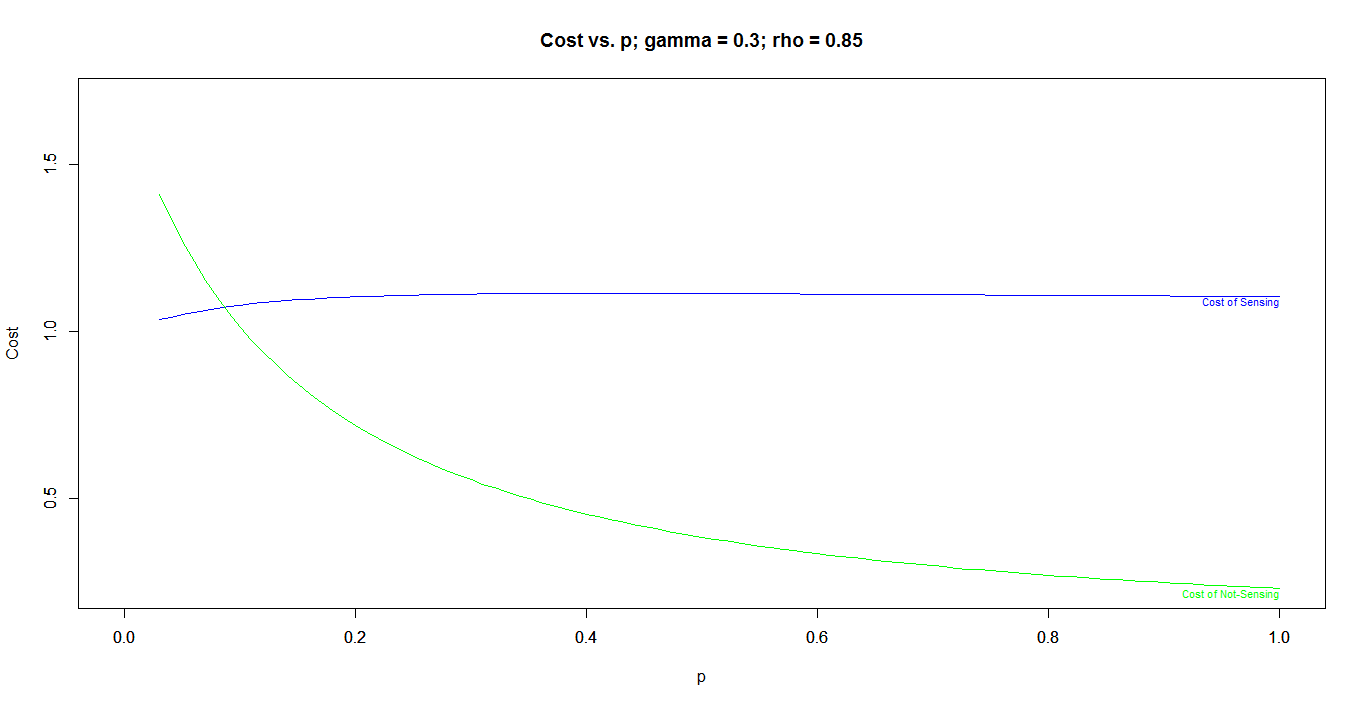
\includegraphics[width=\textwidth]{cost_vs_p_05_085}
		\caption{$\gamma=0.5;\quad\rho=0.85$}
		\label{cost_vs_p_05_085}
	\end{subfigure}
          
	\begin{subfigure}[b]{0.49\textwidth}
	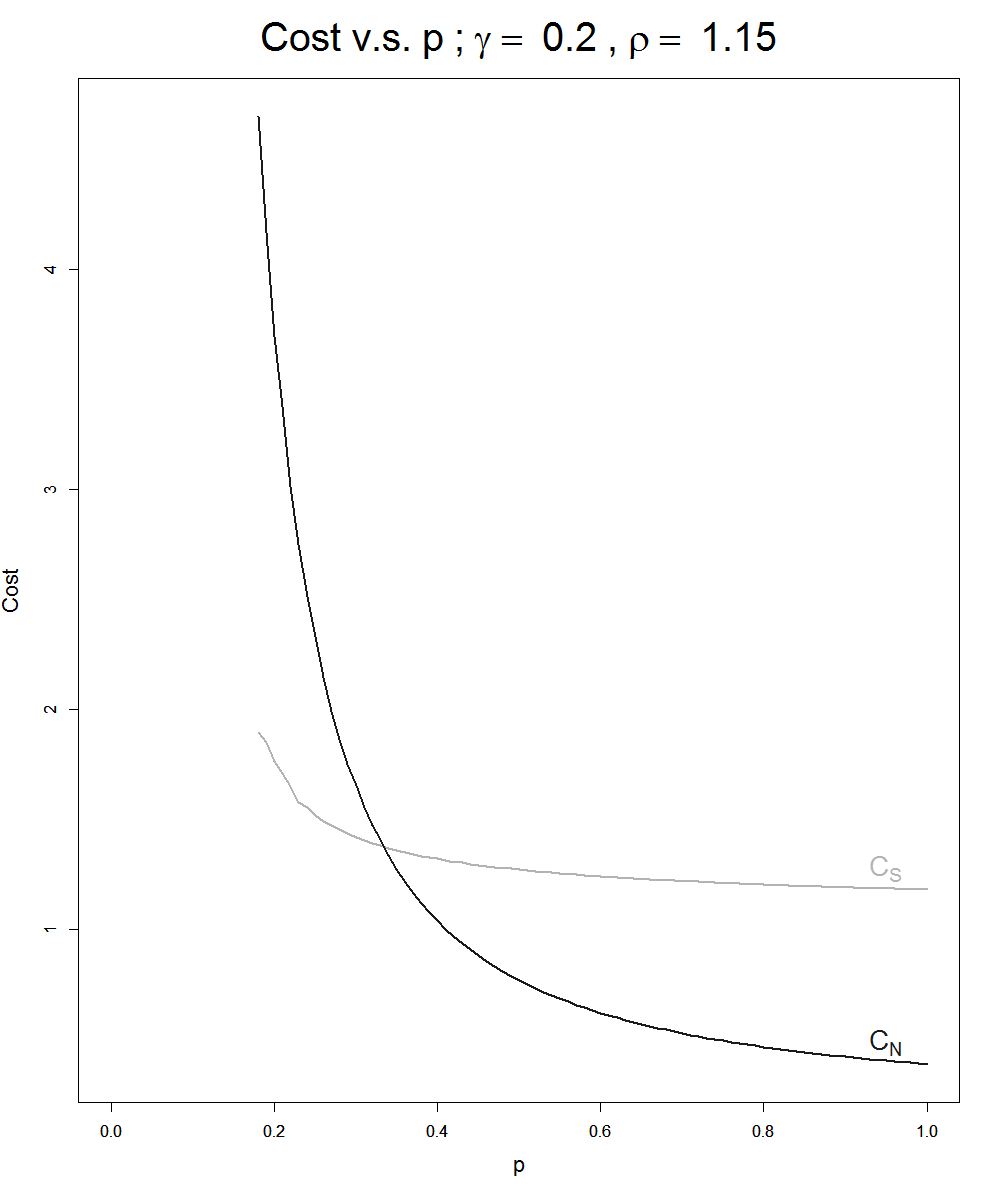
\includegraphics[width=\textwidth]{cost_vs_p_02_115}
		\caption{$\gamma=0.2;\quad\rho=1.15$}
		\label{cost_vs_p_02_115}
	\end{subfigure}
	\begin{subfigure}[b]{0.49\textwidth}
	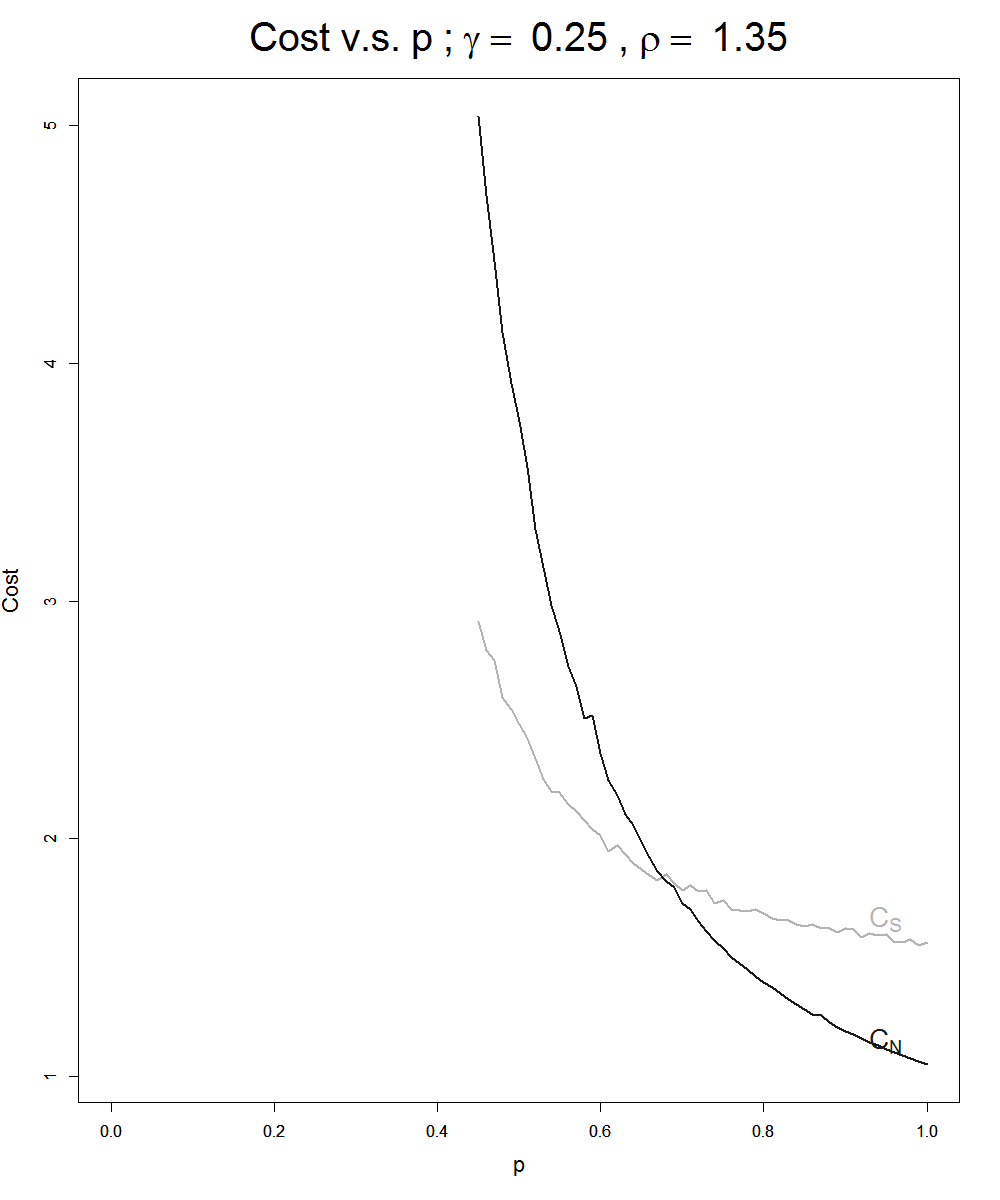
\includegraphics[width=\textwidth]{cost_vs_p_025_135}
		\caption{$\gamma=0.25;\quad\rho=1.35$}
		\label{cost_vs_p_025_135}
	\end{subfigure}
	\caption{The expected costs of sensing and not sensing as a function of $p$ cosidering various values values of $\rho$ and $\gamma$.}\label{CostVsP}
\end{figure}

\newpage
\begin{thebibliography}{99}

%\bibitem{Adiri} Adiri, Igal and Uri Yechiali,
%Optimal priority purchasing and pricing decisions in
%nonmonpoly and monopoly queues, {\it Operations Research}, 22 (1974), 1051-1066.
%
%\bibitem{AlAthari} Al-Athari, Faris Muslim,
%Estimation on the Mean of Truncated Exponential Distribution, {\it Journal of Mathematics and Statistics}, 4 (2008), 284-288.
%
%\bibitem{Allon} Allon, Gad, Achal Bassamboo and Itay Gurvich,
%"We Will be Right with You": Managing Customers with Vague Promises and Cheap 
%Talk, {\it Operations Research}, 59 (2011), 1382-1394.
%
%\bibitem{Alperstein} Alperstein H.,
%Optimal pricing policy for the service facility offering a set of priority
%prices, {\it Management Science}, 34 (1988), 666-671.
%
%\bibitem{Altman} Altman, Eitan and Tania Jimenez,
%Admission Control to an M/M/1 Queue with Partial Information, {\it Lecture Notes in Computer Science}, 7984 (2013), 12-21.
%
%\bibitem{ChenFrank} Chen, Hong and Murray Frank, State dependent pricing with a queue,  {\it IIE Transactions}, 33 (2001), 847-860.

\end{thebibliography}



\end{document}
